\chapter{Građa uređaja}
\label{pog:structure}

Sustav se sastoji od dva uređaja koji zajedno rade u prikupljanju i obradi podataka. \textit{Središnji uređaj} služi za snimanje, obradu i pohranu glasovnih podataka te obradu i pohranu fizioloških signala. Za snimanje fizioloških signala koristi se vlastito projektirana \textit{narukvica}. Središnji uređaj i narukvica razmjenjuju podatke i naredbe putem Bluetooth protokola. Prikupljeni podaci se obrađuju s pomoću neuronske mreže koja se izvodi u stvarnom vremenu na mikrokontroleru, kako bi se utvrdio intenzitet mucanja. Blok dijagram sustava prikazan je na slici \ref{slk:BD_MAIN}.
\begin{figure}[htb]
    \centering
    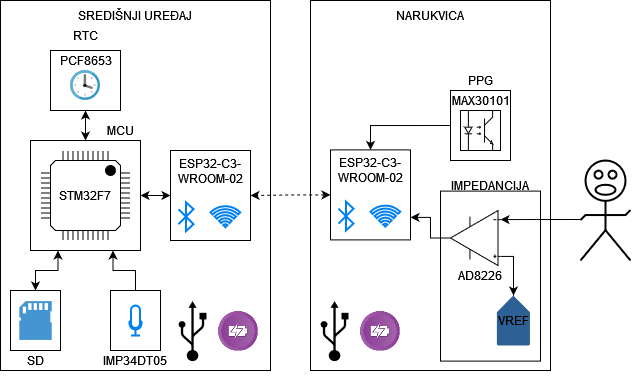
\includegraphics[width=\textwidth]{Figures/block_diagram.drawio.png}
    \caption{Blok dijagram sustava}
    \label{slk:BD_MAIN}
\end{figure}

Na središnjem uređaju nalazi se mikrokontroler (engl. \textit{Microcontroller Unit}, MCU) za obradu podataka, MEMS mikrofon za snimanje govora korisnika, SD kartica za lokalnu pohranu podataka i integrirani sklop za praćenje vremena (engl. \textit{Real Time Clock}, RTC) za vremensku sinkronizaciju snimljenih govornih podataka i biomedicinskih podataka. Podaci će se pohranjivati lokalno na uređaj (SD karticu) kako bi logoped mogao kasnije preuzeti podatke te ih analizirati. Pri tome je važno napomenuti ulogu neuronske mreže na mikrokontroleru, koja može razlikovati korektan govor od mucanja te se izlaz iz neuronske mreže pohranjuje umjesto zvuka, kako bi se izbjegli mogući pravni problemi vezani uz privatnost osoba koje se mogu snimiti skupa s ispitanikom. Upravo je navedeni problem privatnosti i glavni razlog zašto se u trenutnoj kliničkih praksi naprosto ne koriste uređaji koji kontinuirano snimaju zvuk u svakodnevnim prilikama u kojima se nalazi ispitanik tijekom praćenja.

Narukvica mjeri brzinu otkucaja srca (engl. \textit{Heart Rate}, HR) putem fotopletizmografskog senzora (engl. \textit{photoplethysmography}, PPG) i impedanciju kože s pomoću instrumentacijskog pojačala. Promjena impedancije kože je dobar pokazatelj stresa kod ispitanika \cite{edr}, a osobe s poremećajem tečnosti govora pokazuju značajno smanjenje brzine otkucaja srca u stresnim situacijama u odnosu na osobe bez takvih poremećaja \cite{ALM2004123}.

Oba uređaja sadržavaju sustav za bežičnu komunikaciju, baterijsko napajanje i mogućnost punjenja. Zbog dobrih karakteristika i uobičajene primjene u sličnim uređajima, koristi se litij-ionska baterija i mogućnost punjenja putem USB-C sučelja.

Zbog zahtjeva na nosivost uređaja, tiskane pločice (engl. \textit{Printed Circuit Board}, PCB) imaju ograničenje na dimenzije, ali s obzirom  da se radi o prototipu uređaji će sadržavati testne točke i dovoljno velike komponente kako bi eventualna prerada pločice bila lakša. Izrađene pločice su uzimale u obzir kompromise da se ispune ta dva zahtjeva.

Najprije je izrađen središnji sustav kako bi se ispitala mogućnost prikupljanja glasovnih podataka i sustav za napajanje, na temelju čega je u drugom koraku izrađena narukvica da bi se upotpunila tražena funkcionalnost sustava.